\documentclass[1p]{elsarticle_modified}
%\bibliographystyle{elsarticle-num}

%\usepackage[colorlinks]{hyperref}
%\usepackage{abbrmath_seonhwa} %\Abb, \Ascr, \Acal ,\Abf, \Afrak
\usepackage{amsfonts}
\usepackage{amssymb}
\usepackage{amsmath}
\usepackage{amsthm}
\usepackage{scalefnt}
\usepackage{amsbsy}
\usepackage{kotex}
\usepackage{caption}
\usepackage{subfig}
\usepackage{color}
\usepackage{graphicx}
\usepackage{xcolor} %% white, black, red, green, blue, cyan, magenta, yellow
\usepackage{float}
\usepackage{setspace}
\usepackage{hyperref}

\usepackage{tikz}
\usetikzlibrary{arrows}

\usepackage{multirow}
\usepackage{array} % fixed length table
\usepackage{hhline}

%%%%%%%%%%%%%%%%%%%%%
\makeatletter
\renewcommand*\env@matrix[1][\arraystretch]{%
	\edef\arraystretch{#1}%
	\hskip -\arraycolsep
	\let\@ifnextchar\new@ifnextchar
	\array{*\c@MaxMatrixCols c}}
\makeatother %https://tex.stackexchange.com/questions/14071/how-can-i-increase-the-line-spacing-in-a-matrix
%%%%%%%%%%%%%%%

\usepackage[normalem]{ulem}

\newcommand{\msout}[1]{\ifmmode\text{\sout{\ensuremath{#1}}}\else\sout{#1}\fi}
%SOURCE: \msout is \stkout macro in https://tex.stackexchange.com/questions/20609/strikeout-in-math-mode

\newcommand{\cancel}[1]{
	\ifmmode
	{\color{red}\msout{#1}}
	\else
	{\color{red}\sout{#1}}
	\fi
}

\newcommand{\add}[1]{
	{\color{blue}\uwave{#1}}
}

\newcommand{\replace}[2]{
	\ifmmode
	{\color{red}\msout{#1}}{\color{blue}\uwave{#2}}
	\else
	{\color{red}\sout{#1}}{\color{blue}\uwave{#2}}
	\fi
}

\newcommand{\Sol}{\mathcal{S}} %segment
\newcommand{\D}{D} %diagram
\newcommand{\A}{\mathcal{A}} %arc


%%%%%%%%%%%%%%%%%%%%%%%%%%%%%5 test

\def\sl{\operatorname{\textup{SL}}(2,\Cbb)}
\def\psl{\operatorname{\textup{PSL}}(2,\Cbb)}
\def\quan{\mkern 1mu \triangleright \mkern 1mu}

\theoremstyle{definition}
\newtheorem{thm}{Theorem}[section]
\newtheorem{prop}[thm]{Proposition}
\newtheorem{lem}[thm]{Lemma}
\newtheorem{ques}[thm]{Question}
\newtheorem{cor}[thm]{Corollary}
\newtheorem{defn}[thm]{Definition}
\newtheorem{exam}[thm]{Example}
\newtheorem{rmk}[thm]{Remark}
\newtheorem{alg}[thm]{Algorithm}

\newcommand{\I}{\sqrt{-1}}
\begin{document}

%\begin{frontmatter}
%
%\title{Boundary parabolic representations of knots up to 8 crossings}
%
%%% Group authors per affiliation:
%\author{Yunhi Cho} 
%\address{Department of Mathematics, University of Seoul, Seoul, Korea}
%\ead{yhcho@uos.ac.kr}
%
%
%\author{Seonhwa Kim} %\fnref{s_kim}}
%\address{Center for Geometry and Physics, Institute for Basic Science, Pohang, 37673, Korea}
%\ead{ryeona17@ibs.re.kr}
%
%\author{Hyuk Kim}
%\address{Department of Mathematical Sciences, Seoul National University, Seoul 08826, Korea}
%\ead{hyukkim@snu.ac.kr}
%
%\author{Seokbeom Yoon}
%\address{Department of Mathematical Sciences, Seoul National University, Seoul, 08826,  Korea}
%\ead{sbyoon15@snu.ac.kr}
%
%\begin{abstract}
%We find all boundary parabolic representation of knots up to 8 crossings.
%
%\end{abstract}
%\begin{keyword}
%    \MSC[2010] 57M25 
%\end{keyword}
%
%\end{frontmatter}

%\linenumbers
%\tableofcontents
%
\newcommand\colored[1]{\textcolor{white}{\rule[-0.35ex]{0.8em}{1.4ex}}\kern-0.8em\color{red} #1}%
%\newcommand\colored[1]{\textcolor{white}{ #1}\kern-2.17ex	\textcolor{white}{ #1}\kern-1.81ex	\textcolor{white}{ #1}\kern-2.15ex\color{red}#1	}

{\Large $\underline{11a_{261}~(K11a_{261})}$}

\setlength{\tabcolsep}{10pt}
\renewcommand{\arraystretch}{1.6}
\vspace{1cm}\begin{tabular}{m{100pt}>{\centering\arraybackslash}m{274pt}}
\multirow{5}{120pt}{
	\centering
	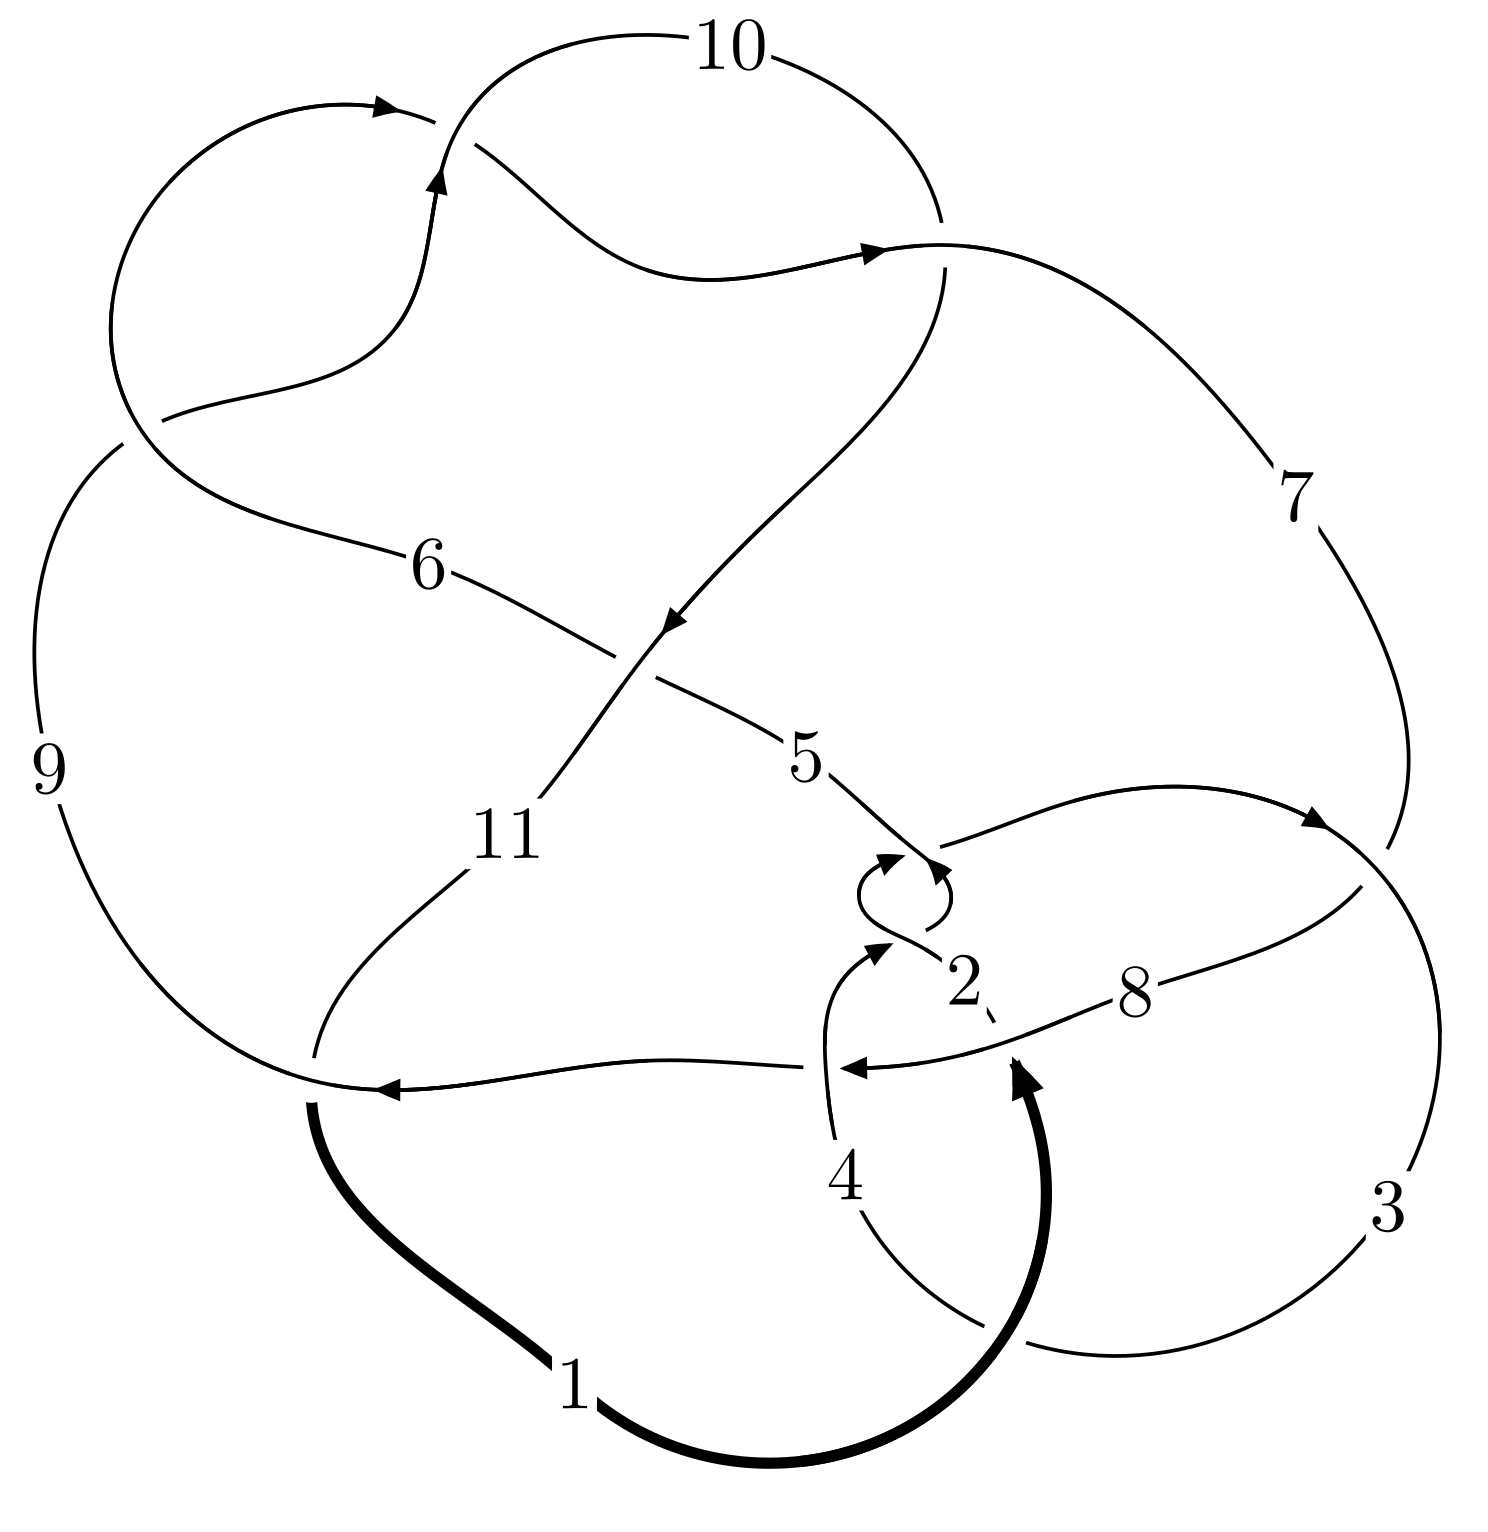
\includegraphics[width=112pt]{../../../GIT/diagram.site/Diagrams/png/510_11a_261.png}\\
\ \ \ A knot diagram\footnotemark}&
\allowdisplaybreaks
\textbf{Linearized knot diagam} \\
\cline{2-2}
 &
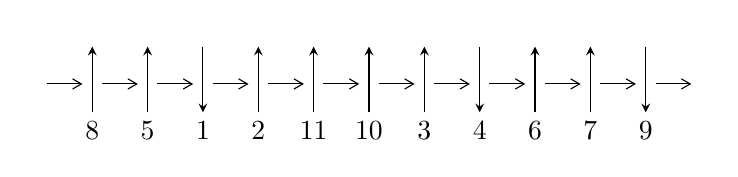
\begin{tikzpicture}[x=20pt, y=17pt]
	% nodes
	\node (C0) at (0, 0) {};
	\node (C1) at (1, 0) {};
	\node (C1U) at (1, +1) {};
	\node (C1D) at (1, -1) {8};

	\node (C2) at (2, 0) {};
	\node (C2U) at (2, +1) {};
	\node (C2D) at (2, -1) {5};

	\node (C3) at (3, 0) {};
	\node (C3U) at (3, +1) {};
	\node (C3D) at (3, -1) {1};

	\node (C4) at (4, 0) {};
	\node (C4U) at (4, +1) {};
	\node (C4D) at (4, -1) {2};

	\node (C5) at (5, 0) {};
	\node (C5U) at (5, +1) {};
	\node (C5D) at (5, -1) {11};

	\node (C6) at (6, 0) {};
	\node (C6U) at (6, +1) {};
	\node (C6D) at (6, -1) {10};

	\node (C7) at (7, 0) {};
	\node (C7U) at (7, +1) {};
	\node (C7D) at (7, -1) {3};

	\node (C8) at (8, 0) {};
	\node (C8U) at (8, +1) {};
	\node (C8D) at (8, -1) {4};

	\node (C9) at (9, 0) {};
	\node (C9U) at (9, +1) {};
	\node (C9D) at (9, -1) {6};

	\node (C10) at (10, 0) {};
	\node (C10U) at (10, +1) {};
	\node (C10D) at (10, -1) {7};

	\node (C11) at (11, 0) {};
	\node (C11U) at (11, +1) {};
	\node (C11D) at (11, -1) {9};
	\node (C12) at (12, 0) {};

	% arrows
	\draw[->,>={angle 60}]
	(C0) edge (C1) (C1) edge (C2) (C2) edge (C3) (C3) edge (C4) (C4) edge (C5) (C5) edge (C6) (C6) edge (C7) (C7) edge (C8) (C8) edge (C9) (C9) edge (C10) (C10) edge (C11) (C11) edge (C12) ;	\draw[->,>=stealth]
	(C1D) edge (C1U) (C2D) edge (C2U) (C3U) edge (C3D) (C4D) edge (C4U) (C5D) edge (C5U) (C6D) edge (C6U) (C7D) edge (C7U) (C8U) edge (C8D) (C9D) edge (C9U) (C10D) edge (C10U) (C11U) edge (C11D) ;
	\end{tikzpicture} \\
\hhline{~~} \\& 
\textbf{Solving Sequence} \\ \cline{2-2} 
 &
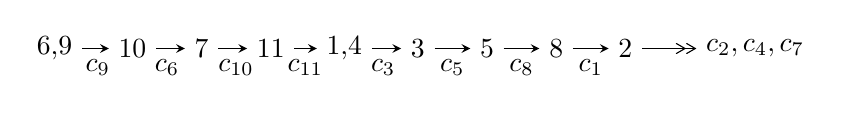
\begin{tikzpicture}[x=25pt, y=7pt]
	% node
	\node (A0) at (-1/8, 0) {6,9};
	\node (A1) at (1, 0) {10};
	\node (A2) at (2, 0) {7};
	\node (A3) at (3, 0) {11};
	\node (A4) at (65/16, 0) {1,4};
	\node (A5) at (41/8, 0) {3};
	\node (A6) at (49/8, 0) {5};
	\node (A7) at (57/8, 0) {8};
	\node (A8) at (65/8, 0) {2};
	\node (C1) at (1/2, -1) {$c_{9}$};
	\node (C2) at (3/2, -1) {$c_{6}$};
	\node (C3) at (5/2, -1) {$c_{10}$};
	\node (C4) at (7/2, -1) {$c_{11}$};
	\node (C5) at (37/8, -1) {$c_{3}$};
	\node (C6) at (45/8, -1) {$c_{5}$};
	\node (C7) at (53/8, -1) {$c_{8}$};
	\node (C8) at (61/8, -1) {$c_{1}$};
	\node (A9) at (10, 0) {$c_{2},c_{4},c_{7}$};

	% edge
	\draw[->,>=stealth]	
	(A0) edge (A1) (A1) edge (A2) (A2) edge (A3) (A3) edge (A4) (A4) edge (A5) (A5) edge (A6) (A6) edge (A7) (A7) edge (A8) ;
	\draw[->>,>={angle 60}]	
	(A8) edge (A9);
\end{tikzpicture} \\ 

\end{tabular} \\

\footnotetext{
The image of knot diagram is generated by the software ``\textbf{Draw programme}" developed by Andrew Bartholomew(\url{http://www.layer8.co.uk/maths/draw/index.htm\#Running-draw}), where we modified some parts for our purpose(\url{https://github.com/CATsTAILs/LinksPainter}).
}\phantom \\ \newline 
\centering \textbf{Ideals for irreducible components\footnotemark of $X_{\text{par}}$} 
 
\begin{align*}
I^u_{1}&=\langle 
-5.81838\times10^{20} u^{64}+3.28868\times10^{20} u^{63}+\cdots+3.16246\times10^{20} b+3.28868\times10^{20},\\
\phantom{I^u_{1}}&\phantom{= \langle  }2.56145\times10^{20} u^{64}+1.23301\times10^{20} u^{63}+\cdots+4.74369\times10^{20} a+1.66504\times10^{21},\;u^{65}-2 u^{64}+\cdots-5 u+1\rangle \\
I^u_{2}&=\langle 
b-1,\;a+1,\;u-1\rangle \\
\\
\end{align*}
\raggedright * 2 irreducible components of $\dim_{\mathbb{C}}=0$, with total 66 representations.\\
\footnotetext{All coefficients of polynomials are rational numbers. But the coefficients are sometimes approximated in decimal forms when there is not enough margin.}
\newpage
\renewcommand{\arraystretch}{1}
\centering \section*{I. $I^u_{1}= \langle -5.82\times10^{20} u^{64}+3.29\times10^{20} u^{63}+\cdots+3.16\times10^{20} b+3.29\times10^{20},\;2.56\times10^{20} u^{64}+1.23\times10^{20} u^{63}+\cdots+4.74\times10^{20} a+1.67\times10^{21},\;u^{65}-2 u^{64}+\cdots-5 u+1 \rangle$}
\flushleft \textbf{(i) Arc colorings}\\
\begin{tabular}{m{7pt} m{180pt} m{7pt} m{180pt} }
\flushright $a_{6}=$&$\begin{pmatrix}0\\u\end{pmatrix}$ \\
\flushright $a_{9}=$&$\begin{pmatrix}1\\0\end{pmatrix}$ \\
\flushright $a_{10}=$&$\begin{pmatrix}1\\- u^2\end{pmatrix}$ \\
\flushright $a_{7}=$&$\begin{pmatrix}u\\- u^3+u\end{pmatrix}$ \\
\flushright $a_{11}=$&$\begin{pmatrix}- u^2+1\\u^4-2 u^2\end{pmatrix}$ \\
\flushright $a_{1}=$&$\begin{pmatrix}- u^4+u^2+1\\u^4-2 u^2\end{pmatrix}$ \\
\flushright $a_{4}=$&$\begin{pmatrix}-0.539970 u^{64}-0.259927 u^{63}+\cdots-1.96576 u-3.51002\\1.83982 u^{64}-1.03991 u^{63}+\cdots+6.70956 u-1.03991\end{pmatrix}$ \\
\flushright $a_{3}=$&$\begin{pmatrix}-0.573322 u^{64}-0.227294 u^{63}+\cdots-0.674829 u-3.39334\\2.04123 u^{64}-1.24062 u^{63}+\cdots+7.59641 u-1.24062\end{pmatrix}$ \\
\flushright $a_{5}=$&$\begin{pmatrix}- u^5+2 u^3- u\\u^7-3 u^5+2 u^3+u\end{pmatrix}$ \\
\flushright $a_{8}=$&$\begin{pmatrix}1.65099 u^{64}-0.842590 u^{63}+\cdots+10.1209 u+2.47153\\-2.24504 u^{64}+1.44254 u^{63}+\cdots-7.30269 u+1.44504\end{pmatrix}$ \\
\flushright $a_{2}=$&$\begin{pmatrix}0.606671 u^{64}+0.193473 u^{63}+\cdots-0.0581858 u+3.37667\\-2.24028 u^{64}+1.44014 u^{63}+\cdots-7.57737 u+1.44014\end{pmatrix}$\\ \flushright $a_{2}=$&$\begin{pmatrix}0.606671 u^{64}+0.193473 u^{63}+\cdots-0.0581858 u+3.37667\\-2.24028 u^{64}+1.44014 u^{63}+\cdots-7.57737 u+1.44014\end{pmatrix}$\\&\end{tabular}
\flushleft \textbf{(ii) Obstruction class $= -1$}\\~\\
\flushleft \textbf{(iii) Cusp Shapes $= \frac{1129105924074689745576}{158123107034570359949} u^{64}-\frac{1258714178007543158198}{158123107034570359949} u^{63}+\cdots+\frac{58838764609619796866}{3364321426267454467} u-\frac{281566083191392405996}{158123107034570359949}$}\\~\\
\newpage\renewcommand{\arraystretch}{1}
\flushleft \textbf{(iv) u-Polynomials at the component}\newline \\
\begin{tabular}{m{50pt}|m{274pt}}
Crossings & \hspace{64pt}u-Polynomials at each crossing \\
\hline $$\begin{aligned}c_{1}\end{aligned}$$&$\begin{aligned}
&u^{65}-4 u^{64}+\cdots- u+1
\end{aligned}$\\
\hline $$\begin{aligned}c_{2},c_{4}\end{aligned}$$&$\begin{aligned}
&u^{65}+2 u^{64}+\cdots-3 u+1
\end{aligned}$\\
\hline $$\begin{aligned}c_{3}\end{aligned}$$&$\begin{aligned}
&u^{65}-11 u^{64}+\cdots+6 u-2
\end{aligned}$\\
\hline $$\begin{aligned}c_{5}\end{aligned}$$&$\begin{aligned}
&u^{65}+3 u^{64}+\cdots-288 u+288
\end{aligned}$\\
\hline $$\begin{aligned}c_{6},c_{9},c_{10}\end{aligned}$$&$\begin{aligned}
&u^{65}-2 u^{64}+\cdots-5 u+1
\end{aligned}$\\
\hline $$\begin{aligned}c_{7}\end{aligned}$$&$\begin{aligned}
&u^{65}+18 u^{63}+\cdots-5599 u+599
\end{aligned}$\\
\hline $$\begin{aligned}c_{8}\end{aligned}$$&$\begin{aligned}
&u^{65}-2 u^{64}+\cdots+875 u+199
\end{aligned}$\\
\hline $$\begin{aligned}c_{11}\end{aligned}$$&$\begin{aligned}
&u^{65}-12 u^{64}+\cdots+15361 u-937
\end{aligned}$\\
\hline
\end{tabular}\\~\\
\newpage\renewcommand{\arraystretch}{1}
\flushleft \textbf{(v) Riley Polynomials at the component}\newline \\
\begin{tabular}{m{50pt}|m{274pt}}
Crossings & \hspace{64pt}Riley Polynomials at each crossing \\
\hline $$\begin{aligned}c_{1}\end{aligned}$$&$\begin{aligned}
&y^{65}-12 y^{64}+\cdots+5 y-1
\end{aligned}$\\
\hline $$\begin{aligned}c_{2},c_{4}\end{aligned}$$&$\begin{aligned}
&y^{65}-48 y^{64}+\cdots+65 y-1
\end{aligned}$\\
\hline $$\begin{aligned}c_{3}\end{aligned}$$&$\begin{aligned}
&y^{65}+9 y^{64}+\cdots-32 y-4
\end{aligned}$\\
\hline $$\begin{aligned}c_{5}\end{aligned}$$&$\begin{aligned}
&y^{65}-15 y^{64}+\cdots+2689344 y-82944
\end{aligned}$\\
\hline $$\begin{aligned}c_{6},c_{9},c_{10}\end{aligned}$$&$\begin{aligned}
&y^{65}-60 y^{64}+\cdots+5 y-1
\end{aligned}$\\
\hline $$\begin{aligned}c_{7}\end{aligned}$$&$\begin{aligned}
&y^{65}+36 y^{64}+\cdots+25490581 y-358801
\end{aligned}$\\
\hline $$\begin{aligned}c_{8}\end{aligned}$$&$\begin{aligned}
&y^{65}+76 y^{64}+\cdots+46837 y-39601
\end{aligned}$\\
\hline $$\begin{aligned}c_{11}\end{aligned}$$&$\begin{aligned}
&y^{65}+40 y^{64}+\cdots+64331905 y-877969
\end{aligned}$\\
\hline
\end{tabular}\\~\\
\newpage\flushleft \textbf{(vi) Complex Volumes and Cusp Shapes}
$$\begin{array}{c|c|c}  
\text{Solutions to }I^u_{1}& \I (\text{vol} + \sqrt{-1}CS) & \text{Cusp shape}\\
 \hline 
\begin{aligned}
u &= \phantom{-}0.678260 + 0.569072 I \\
a &= -0.016122 + 0.492515 I \\
b &= \phantom{-}0.137240 - 0.682876 I\end{aligned}
 & \phantom{-}4.77180 + 0.79551 I & \phantom{-}17.2605 - 1.0216 I \\ \hline\begin{aligned}
u &= \phantom{-}0.678260 - 0.569072 I \\
a &= -0.016122 - 0.492515 I \\
b &= \phantom{-}0.137240 + 0.682876 I\end{aligned}
 & \phantom{-}4.77180 - 0.79551 I & \phantom{-}17.2605 + 1.0216 I \\ \hline\begin{aligned}
u &= \phantom{-}1.14092\phantom{ +0.000000I} \\
a &= -0.115125\phantom{ +0.000000I} \\
b &= \phantom{-}0.758312\phantom{ +0.000000I}\end{aligned}
 & \phantom{-}1.93638\phantom{ +0.000000I} & \phantom{-0.000000 } 0 \\ \hline\begin{aligned}
u &= \phantom{-}0.382954 + 0.760163 I \\
a &= \phantom{-}0.794021 + 0.280590 I \\
b &= \phantom{-}0.046721 - 0.656714 I\end{aligned}
 & \phantom{-}3.78970 + 3.79443 I & \phantom{-}12.5834 - 7.8440 I \\ \hline\begin{aligned}
u &= \phantom{-}0.382954 - 0.760163 I \\
a &= \phantom{-}0.794021 - 0.280590 I \\
b &= \phantom{-}0.046721 + 0.656714 I\end{aligned}
 & \phantom{-}3.78970 - 3.79443 I & \phantom{-}12.5834 + 7.8440 I \\ \hline\begin{aligned}
u &= \phantom{-}1.125870 + 0.332132 I \\
a &= -0.689757 + 0.119579 I \\
b &= \phantom{-}0.687361 + 0.619577 I\end{aligned}
 & \phantom{-}2.88797 - 1.12159 I & \phantom{-0.000000 } 0 \\ \hline\begin{aligned}
u &= \phantom{-}1.125870 - 0.332132 I \\
a &= -0.689757 - 0.119579 I \\
b &= \phantom{-}0.687361 - 0.619577 I\end{aligned}
 & \phantom{-}2.88797 + 1.12159 I & \phantom{-0.000000 } 0 \\ \hline\begin{aligned}
u &= -0.614901 + 0.535330 I \\
a &= -0.761912 + 0.631452 I \\
b &= \phantom{-}0.88334 - 1.27623 I\end{aligned}
 & \phantom{-}5.66757 + 7.97706 I & \phantom{-}9.36287 - 3.39629 I \\ \hline\begin{aligned}
u &= -0.614901 - 0.535330 I \\
a &= -0.761912 - 0.631452 I \\
b &= \phantom{-}0.88334 + 1.27623 I\end{aligned}
 & \phantom{-}5.66757 - 7.97706 I & \phantom{-}9.36287 + 3.39629 I \\ \hline\begin{aligned}
u &= -0.366460 + 0.727085 I \\
a &= -1.42890 + 1.39175 I \\
b &= -0.95536 - 1.32953 I\end{aligned}
 & \phantom{-}4.76852 - 12.28510 I & \phantom{-}7.44035 + 8.76560 I\\
 \hline 
 \end{array}$$\newpage$$\begin{array}{c|c|c}  
\text{Solutions to }I^u_{1}& \I (\text{vol} + \sqrt{-1}CS) & \text{Cusp shape}\\
 \hline 
\begin{aligned}
u &= -0.366460 - 0.727085 I \\
a &= -1.42890 - 1.39175 I \\
b &= -0.95536 + 1.32953 I\end{aligned}
 & \phantom{-}4.76852 + 12.28510 I & \phantom{-}7.44035 - 8.76560 I \\ \hline\begin{aligned}
u &= -1.191650 + 0.175560 I \\
a &= -0.880003 + 0.405987 I \\
b &= -0.699401 - 0.545647 I\end{aligned}
 & \phantom{-}0.37120 - 4.07451 I & \phantom{-0.000000 } 0 \\ \hline\begin{aligned}
u &= -1.191650 - 0.175560 I \\
a &= -0.880003 - 0.405987 I \\
b &= -0.699401 + 0.545647 I\end{aligned}
 & \phantom{-}0.37120 + 4.07451 I & \phantom{-0.000000 } 0 \\ \hline\begin{aligned}
u &= \phantom{-}1.235000 + 0.041141 I \\
a &= -0.79341 - 1.31957 I \\
b &= \phantom{-}0.31476 + 2.40619 I\end{aligned}
 & \phantom{-}3.95963 + 0.42107 I & \phantom{-0.000000 } 0 \\ \hline\begin{aligned}
u &= \phantom{-}1.235000 - 0.041141 I \\
a &= -0.79341 + 1.31957 I \\
b &= \phantom{-}0.31476 - 2.40619 I\end{aligned}
 & \phantom{-}3.95963 - 0.42107 I & \phantom{-0.000000 } 0 \\ \hline\begin{aligned}
u &= \phantom{-}0.049713 + 0.754423 I \\
a &= -0.714482 + 0.300281 I \\
b &= -0.855140 + 0.797416 I\end{aligned}
 & -0.40517 + 5.06438 I & \phantom{-}3.95497 - 7.18299 I \\ \hline\begin{aligned}
u &= \phantom{-}0.049713 - 0.754423 I \\
a &= -0.714482 - 0.300281 I \\
b &= -0.855140 - 0.797416 I\end{aligned}
 & -0.40517 - 5.06438 I & \phantom{-}3.95497 + 7.18299 I \\ \hline\begin{aligned}
u &= -0.339899 + 0.663108 I \\
a &= \phantom{-}1.64239 - 1.16141 I \\
b &= \phantom{-}0.781935 + 0.829638 I\end{aligned}
 & \phantom{-}0.09522 - 6.44593 I & \phantom{-}5.03058 + 9.01119 I \\ \hline\begin{aligned}
u &= -0.339899 - 0.663108 I \\
a &= \phantom{-}1.64239 + 1.16141 I \\
b &= \phantom{-}0.781935 - 0.829638 I\end{aligned}
 & \phantom{-}0.09522 + 6.44593 I & \phantom{-}5.03058 - 9.01119 I \\ \hline\begin{aligned}
u &= -1.235770 + 0.297333 I \\
a &= \phantom{-}0.406289 - 1.235280 I \\
b &= \phantom{-}0.943698 + 0.958823 I\end{aligned}
 & \phantom{-}3.56058 - 8.86995 I & \phantom{-0.000000 } 0\\
 \hline 
 \end{array}$$\newpage$$\begin{array}{c|c|c}  
\text{Solutions to }I^u_{1}& \I (\text{vol} + \sqrt{-1}CS) & \text{Cusp shape}\\
 \hline 
\begin{aligned}
u &= -1.235770 - 0.297333 I \\
a &= \phantom{-}0.406289 + 1.235280 I \\
b &= \phantom{-}0.943698 - 0.958823 I\end{aligned}
 & \phantom{-}3.56058 + 8.86995 I & \phantom{-0.000000 } 0 \\ \hline\begin{aligned}
u &= -0.380812 + 0.610143 I \\
a &= \phantom{-}0.06444 + 1.61329 I \\
b &= -0.058355 - 0.809391 I\end{aligned}
 & \phantom{-}4.44968 - 3.80628 I & \phantom{-}12.2239 + 7.2828 I \\ \hline\begin{aligned}
u &= -0.380812 - 0.610143 I \\
a &= \phantom{-}0.06444 - 1.61329 I \\
b &= -0.058355 + 0.809391 I\end{aligned}
 & \phantom{-}4.44968 + 3.80628 I & \phantom{-}12.2239 - 7.2828 I \\ \hline\begin{aligned}
u &= -1.288300 + 0.091889 I \\
a &= \phantom{-}0.31534 - 2.36850 I \\
b &= \phantom{-}0.348122 + 0.973758 I\end{aligned}
 & \phantom{-}5.10270 - 3.01321 I & \phantom{-0.000000 } 0 \\ \hline\begin{aligned}
u &= -1.288300 - 0.091889 I \\
a &= \phantom{-}0.31534 + 2.36850 I \\
b &= \phantom{-}0.348122 - 0.973758 I\end{aligned}
 & \phantom{-}5.10270 + 3.01321 I & \phantom{-0.000000 } 0 \\ \hline\begin{aligned}
u &= \phantom{-}1.283700 + 0.210832 I \\
a &= \phantom{-}0.005363 - 0.773420 I \\
b &= -0.480767 - 0.212588 I\end{aligned}
 & \phantom{-}1.09839 + 1.94254 I & \phantom{-0.000000 } 0 \\ \hline\begin{aligned}
u &= \phantom{-}1.283700 - 0.210832 I \\
a &= \phantom{-}0.005363 + 0.773420 I \\
b &= -0.480767 + 0.212588 I\end{aligned}
 & \phantom{-}1.09839 - 1.94254 I & \phantom{-0.000000 } 0 \\ \hline\begin{aligned}
u &= -0.419028 + 0.549280 I \\
a &= -1.77640 + 1.52917 I \\
b &= \phantom{-}0.042992 - 0.667229 I\end{aligned}
 & \phantom{-}4.67294 + 0.09706 I & \phantom{-}13.36415 + 0.53030 I \\ \hline\begin{aligned}
u &= -0.419028 - 0.549280 I \\
a &= -1.77640 - 1.52917 I \\
b &= \phantom{-}0.042992 + 0.667229 I\end{aligned}
 & \phantom{-}4.67294 - 0.09706 I & \phantom{-}13.36415 - 0.53030 I \\ \hline\begin{aligned}
u &= \phantom{-}0.301362 + 0.621548 I \\
a &= -0.934672 - 0.857687 I \\
b &= -0.837815 + 0.659025 I\end{aligned}
 & \phantom{-}0.29568 + 2.24337 I & \phantom{-}4.30616 - 2.82871 I\\
 \hline 
 \end{array}$$\newpage$$\begin{array}{c|c|c}  
\text{Solutions to }I^u_{1}& \I (\text{vol} + \sqrt{-1}CS) & \text{Cusp shape}\\
 \hline 
\begin{aligned}
u &= \phantom{-}0.301362 - 0.621548 I \\
a &= -0.934672 + 0.857687 I \\
b &= -0.837815 - 0.659025 I\end{aligned}
 & \phantom{-}0.29568 - 2.24337 I & \phantom{-}4.30616 + 2.82871 I \\ \hline\begin{aligned}
u &= -1.31305\phantom{ +0.000000I} \\
a &= \phantom{-}2.73258\phantom{ +0.000000I} \\
b &= -0.192967\phantom{ +0.000000I}\end{aligned}
 & \phantom{-}6.69568\phantom{ +0.000000I} & \phantom{-0.000000 } 0 \\ \hline\begin{aligned}
u &= -0.492722 + 0.447883 I \\
a &= -0.018732 - 0.417872 I \\
b &= -0.662214 + 0.833663 I\end{aligned}
 & \phantom{-}0.86536 + 2.71020 I & \phantom{-}7.15754 - 3.04555 I \\ \hline\begin{aligned}
u &= -0.492722 - 0.447883 I \\
a &= -0.018732 + 0.417872 I \\
b &= -0.662214 - 0.833663 I\end{aligned}
 & \phantom{-}0.86536 - 2.71020 I & \phantom{-}7.15754 + 3.04555 I \\ \hline\begin{aligned}
u &= \phantom{-}0.345537 + 0.561912 I \\
a &= \phantom{-}3.53045 + 1.22785 I \\
b &= -0.07014 - 3.28534 I\end{aligned}
 & \phantom{-}2.29780 + 1.66494 I & -17.5253 + 6.6293 I \\ \hline\begin{aligned}
u &= \phantom{-}0.345537 - 0.561912 I \\
a &= \phantom{-}3.53045 - 1.22785 I \\
b &= -0.07014 + 3.28534 I\end{aligned}
 & \phantom{-}2.29780 - 1.66494 I & -17.5253 - 6.6293 I \\ \hline\begin{aligned}
u &= -0.051518 + 0.628248 I \\
a &= \phantom{-}1.04887 - 0.98256 I \\
b &= \phantom{-}0.564358 - 0.403906 I\end{aligned}
 & -3.01841 + 1.08766 I & -2.25646 - 1.14539 I \\ \hline\begin{aligned}
u &= -0.051518 - 0.628248 I \\
a &= \phantom{-}1.04887 + 0.98256 I \\
b &= \phantom{-}0.564358 + 0.403906 I\end{aligned}
 & -3.01841 - 1.08766 I & -2.25646 + 1.14539 I \\ \hline\begin{aligned}
u &= -1.41925 + 0.19367 I \\
a &= \phantom{-}1.52410 - 1.19809 I \\
b &= -0.66039 + 1.31268 I\end{aligned}
 & \phantom{-}6.55173 - 3.43032 I & \phantom{-0.000000 } 0 \\ \hline\begin{aligned}
u &= -1.41925 - 0.19367 I \\
a &= \phantom{-}1.52410 + 1.19809 I \\
b &= -0.66039 - 1.31268 I\end{aligned}
 & \phantom{-}6.55173 + 3.43032 I & \phantom{-0.000000 } 0\\
 \hline 
 \end{array}$$\newpage$$\begin{array}{c|c|c}  
\text{Solutions to }I^u_{1}& \I (\text{vol} + \sqrt{-1}CS) & \text{Cusp shape}\\
 \hline 
\begin{aligned}
u &= \phantom{-}0.358057 + 0.432304 I \\
a &= -0.856983 + 0.012393 I \\
b &= \phantom{-}0.337227 + 0.939608 I\end{aligned}
 & \phantom{-}0.927115 + 0.969009 I & \phantom{-}7.33388 - 5.10467 I \\ \hline\begin{aligned}
u &= \phantom{-}0.358057 - 0.432304 I \\
a &= -0.856983 - 0.012393 I \\
b &= \phantom{-}0.337227 - 0.939608 I\end{aligned}
 & \phantom{-}0.927115 - 0.969009 I & \phantom{-}7.33388 + 5.10467 I \\ \hline\begin{aligned}
u &= -1.42039 + 0.24290 I \\
a &= -0.13396 - 1.83660 I \\
b &= \phantom{-}1.027690 + 0.777107 I\end{aligned}
 & \phantom{-}5.81492 - 5.42387 I & \phantom{-0.000000 } 0 \\ \hline\begin{aligned}
u &= -1.42039 - 0.24290 I \\
a &= -0.13396 + 1.83660 I \\
b &= \phantom{-}1.027690 - 0.777107 I\end{aligned}
 & \phantom{-}5.81492 + 5.42387 I & \phantom{-0.000000 } 0 \\ \hline\begin{aligned}
u &= -1.43036 + 0.22015 I \\
a &= -2.83053 + 4.42260 I \\
b &= -0.01146 - 3.25716 I\end{aligned}
 & \phantom{-}7.99318 - 4.57389 I & \phantom{-0.000000 } 0 \\ \hline\begin{aligned}
u &= -1.43036 - 0.22015 I \\
a &= -2.83053 - 4.42260 I \\
b &= -0.01146 + 3.25716 I\end{aligned}
 & \phantom{-}7.99318 + 4.57389 I & \phantom{-0.000000 } 0 \\ \hline\begin{aligned}
u &= \phantom{-}1.43947 + 0.17545 I \\
a &= -0.61970 - 1.47828 I \\
b &= \phantom{-}0.652456 + 0.963631 I\end{aligned}
 & \phantom{-}6.93022 - 0.40426 I & \phantom{-0.000000 } 0 \\ \hline\begin{aligned}
u &= \phantom{-}1.43947 - 0.17545 I \\
a &= -0.61970 + 1.47828 I \\
b &= \phantom{-}0.652456 - 0.963631 I\end{aligned}
 & \phantom{-}6.93022 + 0.40426 I & \phantom{-0.000000 } 0 \\ \hline\begin{aligned}
u &= \phantom{-}1.43628 + 0.25338 I \\
a &= -0.74240 - 2.08871 I \\
b &= -0.828861 + 0.874237 I\end{aligned}
 & \phantom{-}5.79461 + 9.79626 I & \phantom{-0.000000 } 0 \\ \hline\begin{aligned}
u &= \phantom{-}1.43628 - 0.25338 I \\
a &= -0.74240 + 2.08871 I \\
b &= -0.828861 - 0.874237 I\end{aligned}
 & \phantom{-}5.79461 - 9.79626 I & \phantom{-0.000000 } 0\\
 \hline 
 \end{array}$$\newpage$$\begin{array}{c|c|c}  
\text{Solutions to }I^u_{1}& \I (\text{vol} + \sqrt{-1}CS) & \text{Cusp shape}\\
 \hline 
\begin{aligned}
u &= \phantom{-}1.44643 + 0.20811 I \\
a &= \phantom{-}1.52474 + 1.92775 I \\
b &= \phantom{-}0.076180 - 0.648466 I\end{aligned}
 & \phantom{-}10.64080 + 2.70423 I & \phantom{-0.000000 } 0 \\ \hline\begin{aligned}
u &= \phantom{-}1.44643 - 0.20811 I \\
a &= \phantom{-}1.52474 - 1.92775 I \\
b &= \phantom{-}0.076180 + 0.648466 I\end{aligned}
 & \phantom{-}10.64080 - 2.70423 I & \phantom{-0.000000 } 0 \\ \hline\begin{aligned}
u &= \phantom{-}1.44458 + 0.23052 I \\
a &= \phantom{-}0.00727 + 2.22521 I \\
b &= -0.008684 - 0.861520 I\end{aligned}
 & \phantom{-}10.31070 + 6.89598 I & \phantom{-0.000000 } 0 \\ \hline\begin{aligned}
u &= \phantom{-}1.44458 - 0.23052 I \\
a &= \phantom{-}0.00727 - 2.22521 I \\
b &= -0.008684 + 0.861520 I\end{aligned}
 & \phantom{-}10.31070 - 6.89598 I & \phantom{-0.000000 } 0 \\ \hline\begin{aligned}
u &= \phantom{-}1.45377 + 0.27698 I \\
a &= \phantom{-}0.60639 + 2.76642 I \\
b &= \phantom{-}0.97235 - 1.38618 I\end{aligned}
 & \phantom{-}10.6167 + 15.9423 I & \phantom{-0.000000 } 0 \\ \hline\begin{aligned}
u &= \phantom{-}1.45377 - 0.27698 I \\
a &= \phantom{-}0.60639 - 2.76642 I \\
b &= \phantom{-}0.97235 + 1.38618 I\end{aligned}
 & \phantom{-}10.6167 - 15.9423 I & \phantom{-0.000000 } 0 \\ \hline\begin{aligned}
u &= -1.46439 + 0.28501 I \\
a &= -0.788256 + 1.075800 I \\
b &= -0.145502 - 0.724051 I\end{aligned}
 & \phantom{-}9.73502 - 7.58811 I & \phantom{-0.000000 } 0 \\ \hline\begin{aligned}
u &= -1.46439 - 0.28501 I \\
a &= -0.788256 - 1.075800 I \\
b &= -0.145502 + 0.724051 I\end{aligned}
 & \phantom{-}9.73502 + 7.58811 I & \phantom{-0.000000 } 0 \\ \hline\begin{aligned}
u &= \phantom{-}1.49064 + 0.14963 I \\
a &= \phantom{-}1.32087 + 1.93888 I \\
b &= -0.77806 - 1.33217 I\end{aligned}
 & \phantom{-}12.49300 - 5.62787 I & \phantom{-0.000000 } 0 \\ \hline\begin{aligned}
u &= \phantom{-}1.49064 - 0.14963 I \\
a &= \phantom{-}1.32087 - 1.93888 I \\
b &= -0.77806 + 1.33217 I\end{aligned}
 & \phantom{-}12.49300 + 5.62787 I & \phantom{-0.000000 } 0\\
 \hline 
 \end{array}$$\newpage$$\begin{array}{c|c|c}  
\text{Solutions to }I^u_{1}& \I (\text{vol} + \sqrt{-1}CS) & \text{Cusp shape}\\
 \hline 
\begin{aligned}
u &= -1.50530 + 0.13452 I \\
a &= \phantom{-}0.26995 + 1.42007 I \\
b &= -0.180993 - 0.917016 I\end{aligned}
 & \phantom{-}11.93110 - 3.09362 I & \phantom{-0.000000 } 0 \\ \hline\begin{aligned}
u &= -1.50530 - 0.13452 I \\
a &= \phantom{-}0.26995 - 1.42007 I \\
b &= -0.180993 + 0.917016 I\end{aligned}
 & \phantom{-}11.93110 + 3.09362 I & \phantom{-0.000000 } 0 \\ \hline\begin{aligned}
u &= \phantom{-}0.113883 + 0.422940 I \\
a &= -1.56859 - 0.39304 I \\
b &= -0.431618 + 1.169140 I\end{aligned}
 & \phantom{-}0.92611 + 1.21767 I & \phantom{-}5.78394 - 3.84378 I \\ \hline\begin{aligned}
u &= \phantom{-}0.113883 - 0.422940 I \\
a &= -1.56859 + 0.39304 I \\
b &= -0.431618 - 1.169140 I\end{aligned}
 & \phantom{-}0.92611 - 1.21767 I & \phantom{-}5.78394 + 3.84378 I \\ \hline\begin{aligned}
u &= \phantom{-}0.242610\phantom{ +0.000000I} \\
a &= -5.62882\phantom{ +0.000000I} \\
b &= \phantom{-}1.13132\phantom{ +0.000000I}\end{aligned}
 & \phantom{-}2.24319\phantom{ +0.000000I} & \phantom{-}1.34300\phantom{ +0.000000I}\\
 \hline 
 \end{array}$$\newpage\newpage\renewcommand{\arraystretch}{1}
\centering \section*{II. $I^u_{2}= \langle b-1,\;a+1,\;u-1 \rangle$}
\flushleft \textbf{(i) Arc colorings}\\
\begin{tabular}{m{7pt} m{180pt} m{7pt} m{180pt} }
\flushright $a_{6}=$&$\begin{pmatrix}0\\1\end{pmatrix}$ \\
\flushright $a_{9}=$&$\begin{pmatrix}1\\0\end{pmatrix}$ \\
\flushright $a_{10}=$&$\begin{pmatrix}1\\-1\end{pmatrix}$ \\
\flushright $a_{7}=$&$\begin{pmatrix}1\\0\end{pmatrix}$ \\
\flushright $a_{11}=$&$\begin{pmatrix}0\\-1\end{pmatrix}$ \\
\flushright $a_{1}=$&$\begin{pmatrix}1\\-1\end{pmatrix}$ \\
\flushright $a_{4}=$&$\begin{pmatrix}-1\\1\end{pmatrix}$ \\
\flushright $a_{3}=$&$\begin{pmatrix}-1\\1\end{pmatrix}$ \\
\flushright $a_{5}=$&$\begin{pmatrix}0\\1\end{pmatrix}$ \\
\flushright $a_{8}=$&$\begin{pmatrix}2\\-1\end{pmatrix}$ \\
\flushright $a_{2}=$&$\begin{pmatrix}-1\\0\end{pmatrix}$\\ \flushright $a_{2}=$&$\begin{pmatrix}-1\\0\end{pmatrix}$\\&\end{tabular}
\flushleft \textbf{(ii) Obstruction class $= 1$}\\~\\
\flushleft \textbf{(iii) Cusp Shapes $= 12$}\\~\\
\newpage\renewcommand{\arraystretch}{1}
\flushleft \textbf{(iv) u-Polynomials at the component}\newline \\
\begin{tabular}{m{50pt}|m{274pt}}
Crossings & \hspace{64pt}u-Polynomials at each crossing \\
\hline $$\begin{aligned}c_{1},c_{4},c_{7}\\c_{8},c_{9},c_{10}\\c_{11}\end{aligned}$$&$\begin{aligned}
&u-1
\end{aligned}$\\
\hline $$\begin{aligned}c_{2},c_{6}\end{aligned}$$&$\begin{aligned}
&u+1
\end{aligned}$\\
\hline $$\begin{aligned}c_{3},c_{5}\end{aligned}$$&$\begin{aligned}
&u
\end{aligned}$\\
\hline
\end{tabular}\\~\\
\newpage\renewcommand{\arraystretch}{1}
\flushleft \textbf{(v) Riley Polynomials at the component}\newline \\
\begin{tabular}{m{50pt}|m{274pt}}
Crossings & \hspace{64pt}Riley Polynomials at each crossing \\
\hline $$\begin{aligned}c_{1},c_{2},c_{4}\\c_{6},c_{7},c_{8}\\c_{9},c_{10},c_{11}\end{aligned}$$&$\begin{aligned}
&y-1
\end{aligned}$\\
\hline $$\begin{aligned}c_{3},c_{5}\end{aligned}$$&$\begin{aligned}
&y
\end{aligned}$\\
\hline
\end{tabular}\\~\\
\newpage\flushleft \textbf{(vi) Complex Volumes and Cusp Shapes}
$$\begin{array}{c|c|c}  
\text{Solutions to }I^u_{2}& \I (\text{vol} + \sqrt{-1}CS) & \text{Cusp shape}\\
 \hline 
\begin{aligned}
u &= \phantom{-}1.00000\phantom{ +0.000000I} \\
a &= -1.00000\phantom{ +0.000000I} \\
b &= \phantom{-}1.00000\phantom{ +0.000000I}\end{aligned}
 & \phantom{-}3.28987\phantom{ +0.000000I} & \phantom{-}12.0000\phantom{ +0.000000I}\\
 \hline 
 \end{array}$$\newpage
\newpage\renewcommand{\arraystretch}{1}
\centering \section*{ III. u-Polynomials}
\begin{tabular}{m{50pt}|m{274pt}}
Crossings & \hspace{64pt}u-Polynomials at each crossing \\
\hline $$\begin{aligned}c_{1}\end{aligned}$$&$\begin{aligned}
&(u-1)(u^{65}-4 u^{64}+\cdots- u+1)
\end{aligned}$\\
\hline $$\begin{aligned}c_{2}\end{aligned}$$&$\begin{aligned}
&(u+1)(u^{65}+2 u^{64}+\cdots-3 u+1)
\end{aligned}$\\
\hline $$\begin{aligned}c_{3}\end{aligned}$$&$\begin{aligned}
&u(u^{65}-11 u^{64}+\cdots+6 u-2)
\end{aligned}$\\
\hline $$\begin{aligned}c_{4}\end{aligned}$$&$\begin{aligned}
&(u-1)(u^{65}+2 u^{64}+\cdots-3 u+1)
\end{aligned}$\\
\hline $$\begin{aligned}c_{5}\end{aligned}$$&$\begin{aligned}
&u(u^{65}+3 u^{64}+\cdots-288 u+288)
\end{aligned}$\\
\hline $$\begin{aligned}c_{6}\end{aligned}$$&$\begin{aligned}
&(u+1)(u^{65}-2 u^{64}+\cdots-5 u+1)
\end{aligned}$\\
\hline $$\begin{aligned}c_{7}\end{aligned}$$&$\begin{aligned}
&(u-1)(u^{65}+18 u^{63}+\cdots-5599 u+599)
\end{aligned}$\\
\hline $$\begin{aligned}c_{8}\end{aligned}$$&$\begin{aligned}
&(u-1)(u^{65}-2 u^{64}+\cdots+875 u+199)
\end{aligned}$\\
\hline $$\begin{aligned}c_{9},c_{10}\end{aligned}$$&$\begin{aligned}
&(u-1)(u^{65}-2 u^{64}+\cdots-5 u+1)
\end{aligned}$\\
\hline $$\begin{aligned}c_{11}\end{aligned}$$&$\begin{aligned}
&(u-1)(u^{65}-12 u^{64}+\cdots+15361 u-937)
\end{aligned}$\\
\hline
\end{tabular}\newpage\renewcommand{\arraystretch}{1}
\centering \section*{ IV. Riley Polynomials}
\begin{tabular}{m{50pt}|m{274pt}}
Crossings & \hspace{64pt}Riley Polynomials at each crossing \\
\hline $$\begin{aligned}c_{1}\end{aligned}$$&$\begin{aligned}
&(y-1)(y^{65}-12 y^{64}+\cdots+5 y-1)
\end{aligned}$\\
\hline $$\begin{aligned}c_{2},c_{4}\end{aligned}$$&$\begin{aligned}
&(y-1)(y^{65}-48 y^{64}+\cdots+65 y-1)
\end{aligned}$\\
\hline $$\begin{aligned}c_{3}\end{aligned}$$&$\begin{aligned}
&y(y^{65}+9 y^{64}+\cdots-32 y-4)
\end{aligned}$\\
\hline $$\begin{aligned}c_{5}\end{aligned}$$&$\begin{aligned}
&y(y^{65}-15 y^{64}+\cdots+2689344 y-82944)
\end{aligned}$\\
\hline $$\begin{aligned}c_{6},c_{9},c_{10}\end{aligned}$$&$\begin{aligned}
&(y-1)(y^{65}-60 y^{64}+\cdots+5 y-1)
\end{aligned}$\\
\hline $$\begin{aligned}c_{7}\end{aligned}$$&$\begin{aligned}
&(y-1)(y^{65}+36 y^{64}+\cdots+2.54906\times10^{7} y-358801)
\end{aligned}$\\
\hline $$\begin{aligned}c_{8}\end{aligned}$$&$\begin{aligned}
&(y-1)(y^{65}+76 y^{64}+\cdots+46837 y-39601)
\end{aligned}$\\
\hline $$\begin{aligned}c_{11}\end{aligned}$$&$\begin{aligned}
&(y-1)(y^{65}+40 y^{64}+\cdots+6.43319\times10^{7} y-877969)
\end{aligned}$\\
\hline
\end{tabular}
\vskip 2pc
\end{document}